
\documentclass[11pt, oneside]{article} 

\usepackage[top=1in, bottom=1in, left=.75in, right=.75in]{geometry} 

\usepackage{graphicx} 
\usepackage{setspace} 
\usepackage{amssymb} 
\usepackage{placeins} 
\usepackage{float} 
\usepackage{amsmath}
\usepackage[hang,small,bf]{caption} 
\usepackage{subcaption}
\usepackage{tikz}
\usepackage{color}


%Headers
\usepackage{fancyhdr} 
\pagestyle{fancy}
\renewcommand{\headrulewidth}{3pt}    % Header line width
\renewcommand{\footrulewidth}{0pt}    % Footer line width 
\lhead{[ECEN 2270]}    
\chead{Robot Dot Printer}
\rhead{John Dunn \& Alex Mault}
\lfoot{\today}
\cfoot{}
\rfoot{Page \thepage} 

%Commands for the tikzpicture
\newcommand\drawServoAssembly{
    \draw[fill = gray] (0,0) rectangle (0.35,0.6);

    \draw[rotate=30,rounded corners=1,fill = white] (0.2,0.15) rectangle (1.3,0.36);
    \draw[rotate=30,rounded corners=1,fill = white] (0.8,0.21) rectangle (1.15,0.3);
    \draw[fill = gray] (0.175,0.4) circle (0.05);
    
    \draw[fill = white,rounded corners = 4] (0.57,-3) rectangle (0.85,0.9);
    \path[fill = black] (0.6,-2.95)--(0.82,-2.95)--(0.7,-3.25)--cycle;
    
    \begin{scope}[shift={(0.71,0.72)},scale = 0.07]
        \drawScrewHead;
    \end{scope}
}
\newcommand\drawScrewHead{
    \draw (0,0) circle (1);
    \draw (0,-0.75)--(0,0.75);
    \draw (-0.75,0)--(0.75,0);
}
\newcommand\drawCross{
    \draw[red,line width=2] (0,0)--(1,1);
    \draw[red,line width=2] (0,1)--(1,0);
}

%Set our title and author varables
%Will be used below by \maketitle
\title{Final Project - Robot Dot Printer} 
\author{John Dunn and Alex Mault} \begin{document}

%-------Beginning of Cover------%
%We want our cover page single spaced
\begin{singlespace}

	\maketitle
	
	
	\begin{center}
		\includegraphics[width=100mm]{Images/printerAss2} 
	\end{center}
	
\end{singlespace}

\newpage
%---------End of Cover-----------%

\section{Introduction}
"Theoretically, this should work" was probably the most commonly used phrase in our final project days. The goal of our final project was to create a robot that is able to print discrete images using sharpies actuated by servo motors. To complete this goal, we had to construct a printer assembly that would be placed on the rear of our robot, and developed code for the Arduino to drive servos with pulse width modulation such that sharpies moved in a linear path.
\begin{figure}[H]
    \centering
    \includegraphics[width = 0.4\textwidth]{Images/BlockDiagram}
    \caption{Block Diagram of our system.}
    \label{fig:blockDiagram}
\end{figure}



\section{Additional Goals: Motor Controller PCB}
An additional goal we had was to create a motor controller PCB that would replace the circuitry from labs 2-4. This would declutter the top of the robot and prevent wires and components from mistakenly coming loose. Even though we constructed the board to the highest possible accuracy, the two sided board shown in Fig. \ref{fig:MotorContPCB} failed to drive the right motor correctly. Due to time constraints, we elected to simply reorganize the original breadboard circuitry from labs 2-4 (Fig. \ref{fig:MotorContBread}).

\begin{figure}[H]
    \centering
    \begin{subfigure}[b]{0.35\textwidth}
        \includegraphics[width = \textwidth]{Images/MotorContPCB}
        \caption{Attempted motor controller 2-sided PCB to replace circuitry.}
        \label{fig:MotorContPCB}
    \end{subfigure}
    \begin{subfigure}[b]{0.35\textwidth}
        \includegraphics[width = \textwidth]{Images/MotorContBread}
        \caption[center]{Functional breadboarded motor controller circuitry.}
        \label{fig:MotorContBread}
    \end{subfigure}
    \caption{Versions of the motor control circuitry.}
    \label{fig:MotorCont}
\end{figure}

Lastly, we had the idea to use a Sparkfun manufactured PWM shield (Fig. \ref{fig:PWMShield})that had the ability to drive the 8 servo motors. Unfortunately, luck was not on our side, because the board had a faulty power management system. To sidestep this issue, we settled for only using 6 servos, which was the maximum the arduino could provide.
\begin{figure}[H]
    \centering
    \begin{subfigure}[b]{0.35\textwidth}
        \includegraphics[width = \textwidth]{Images/PWMShield}
        \caption{Faulty Sparkfun PWM shield.}
        \label{fig:PWMShield}
    \end{subfigure}
    \begin{subfigure}[b]{0.35\textwidth}
        \includegraphics[width = \textwidth]{Images/PWMArd}
        \caption[center]{The reliable Arduino PWM.}
        \label{fig:PWMArd}
    \end{subfigure}
    \caption{Versions of the Pulse Width Modulation.}
    \label{fig:PWM}
\end{figure}
%Include block diagram
\section{Design of Printer Assembly}
Next, something that actually worked! Originally we had planned on using solenoids to actuate the Sharpies. After connection between the solenoids and markers became a  dubious prospect at best, we opted for a more accurate, and more Arduino friendly method of actuation, the humble sub-micro servo. The servos allowed us to use PWM to accurately push and pull the Sharpies.

The first issue we ran across was constructing servo horns to connect servo and Sharpie. Using a laser cutter and some 1/8" acrylic, we were able to manufacture horns that fit our application wonderfully. A slot was cut along the length of the arm which allowed the Sharpie to side back and forth on its vertical path. This movement minimized the torque on the servo motors.


\begin{figure}[H]
    \centering
    \begin{subfigure}[b]{0.38\textwidth}
        \centering
        \includegraphics[width = \textwidth]{Images/servoHorn}
        \caption{Sub-micro servo (upper left), and laser cut servo horn (right).}
        \label{fig:servoHorn}
    \end{subfigure}
    \begin{subfigure}[b]{0.3\textwidth}
        \includegraphics[width = \textwidth]{Images/explodeServo}
        \caption{Connection between Sharpie and servo.}
        \label{fig:explodeServo}
    \end{subfigure}
    \begin{subfigure}[b]{0.3\textwidth}
        \includegraphics[width = \textwidth]{Images/attachedServo}
        \caption[center]{Attached servo and Sharpie assembly.}
        \label{fig:attachedServo}
    \end{subfigure}
    \caption{Servo-Sharpie Assembly.}
    \label{fig:ServSharpAss}
\end{figure}
 

\begin{figure}[H]
    \centering
    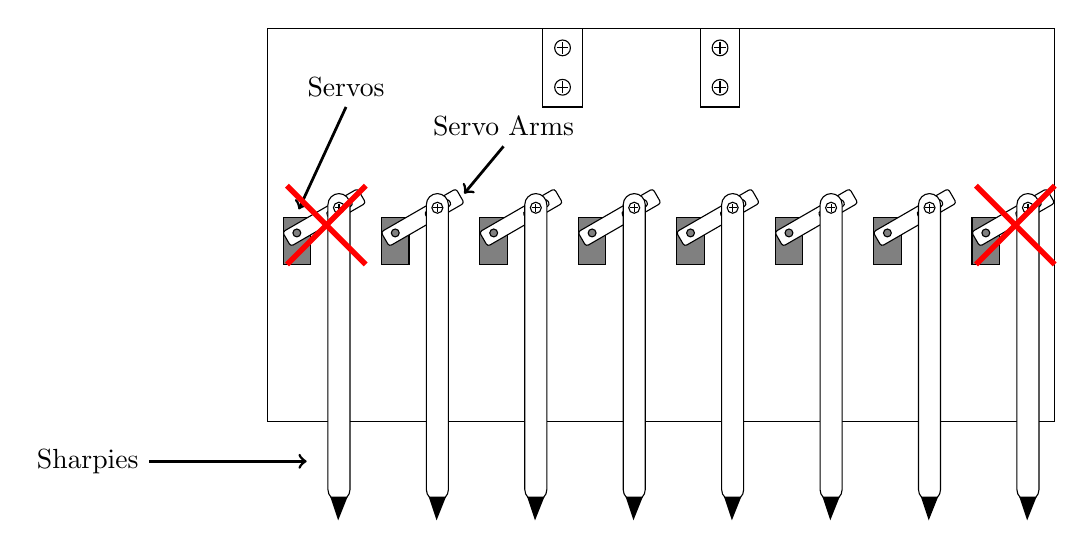
\begin{tikzpicture}[scale = 1]
        \draw (-10,0) rectangle (0,5);
        \foreach \xoffset in {-10,-8.75,-7.5,-6.25,-5,-3.75,-2.5,-1.25}
        {
            \begin{scope}[shift={(\xoffset+0.2,2)}]
                \drawServoAssembly;
            \end{scope}
        }
        \draw (-6.5,4) rectangle (-6,5);
        \draw (-4.5,4) rectangle (-4,5);
        \draw[->,line width = 1] (-11.5,-0.5)--(-9.5,-0.5) node[left,pos=0] {Sharpies};
        \draw[->,line width = 1] (-9,4)--(-9.6,2.7) node[above,pos=0] {Servos};
        \draw[->,line width = 1] (-7,3.5)--(-7.5,2.9) node[above,pos=0] {Servo Arms};
        
        \foreach \xoffset in {-62.5,-42.5}{
            \foreach \yoffset in {47.5,42.5}{
                \begin{scope}[scale = 0.1, shift = {(\xoffset,\yoffset)}]
                    \drawScrewHead;
                \end{scope}
            }
        }
        \foreach \xoffset in {-9.75,-1}{
            \begin{scope}[shift = {(\xoffset, 2)}]
                \drawCross;
            \end{scope}
        }
    \end{tikzpicture}
    \caption{Printer Assembly. Due to the buggy nature of the PWM shield, we decided to remove the outside servo assemblies in favor of using the built-in PWM outputs of the Arduino.}
    \label{fig:PrintAssFront}
\end{figure}
\begin{figure}[H]
    \centering
    \begin{subfigure}[b]{0.4\textwidth}
        \centering
        \includegraphics[width = \textwidth]{Images/printerAss1}
        \caption{Construction of printer assembly.}
        \label{fig:printerAss1}
    \end{subfigure}
    \begin{subfigure}[b]{0.38\textwidth}
        \includegraphics[width = \textwidth]{Images/printerAss2}
        \caption{Completed printer assembly.}
        \label{fig:printerAss2}
    \end{subfigure}
    \caption{Printer assembly. By laser cutting the printer assembly, the servos were able to be press fit into the holes without any screws. This accuracy was accomplished through many iterations.}
    \label{fig:printerAss2}
\end{figure}
\section{PWM Servo Control}
Servos are controlled by pulse width modulation. Different pulse widths are associated with different positions, shown in Fig. \ref{fig:servoPWM}. In our robot, we use three positions: Storage (fully up), Set (down but not touching), and Print (down and touching). We ran across issues with power regulation when we tried to drive all 8 servos from PWM shield, so we defaulted to using the six PWM pins available on the Arduino. However, eight PWM outputs were required to control the  six servos and two robot wheels. Two additional PWM outputs were made by manipulating Arduino digital output pins with strategic timer interrupts. This created a PWM signal suitable to be a voltage reference to the robot motor controller.

\begin{figure}[H]
    \centering
    \includegraphics[width = 0.6\textwidth]{Images/PWM}
    \caption{Explanation of pulse width modulation with servos.}
    \label{fig:servoPWM}
\end{figure}

In order to print designs, servos would have to be in specific positions at specific times. The process of printing would be to 1) Push Sharpies down, 2) Move forward, 3) Change positions of Sharpies, 4) Repeat. Using a linked list method explained graphically in Fig. 

\begin{figure}[H]
    \centering
    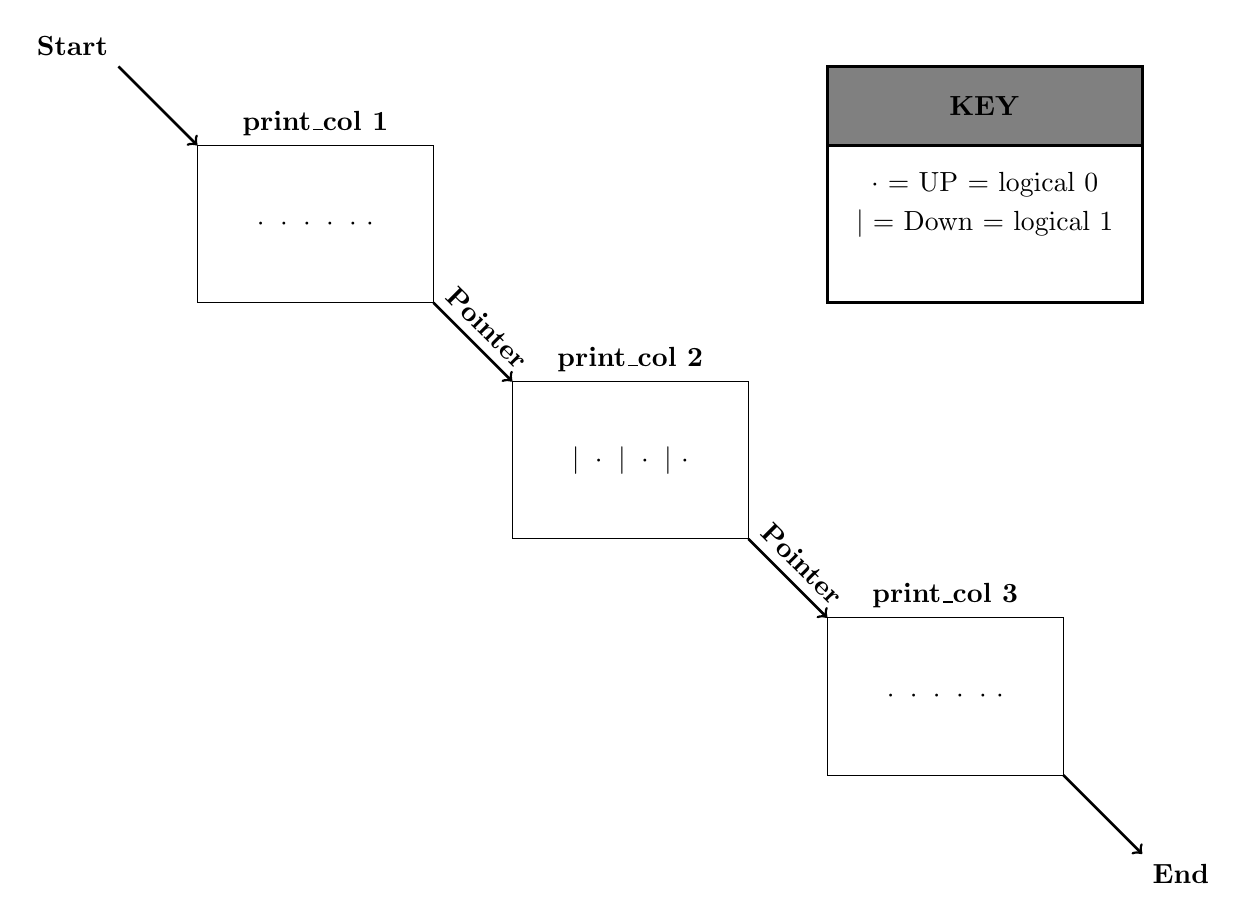
\begin{tikzpicture}
        \draw[->, line width =1] (0,10) -- (1,9) node[above left, pos = 0] {\textbf{Start}};
        \draw (1,7) rectangle (4,9) node at (2.5,8) {$\cdot~\cdot~\cdot~\cdot~\cdot~\cdot$};
        \node[above] at (2.5,9) {\textbf{print\_col 1}};
        \draw[->, line width = 1] (4,7) -- (5,6) node[sloped, pos = 0.5, above] {\textbf{Pointer}};
        \draw (5,4) rectangle (8,6) node at (6.5,5) {$|~\cdot~|~\cdot~|~\cdot$};
        \node[above] at (6.5,6) {\textbf{print\_col 2}};
        \draw[->, line width = 1] (8,4) -- (9,3) node[sloped, pos = 0.5, above] {\textbf{Pointer}};
        \draw (9,1) rectangle (12,3) node at (10.5,2) {$\cdot~\cdot~\cdot~\cdot~\cdot~\cdot$};
        \node[above] at (10.5,3) {\textbf{print\_col 3}};
        \draw[->, line width =1] (12,1) -- (13,0) node[below right, pos = 1] {\textbf{End}};
        
        \path[fill = gray] (9,9)--(9,10)--(13,10)--(13,9)--cycle;        
        \draw[line width = 1] (9,7) rectangle (13,10);
        \draw[line width = 1] (9,9) -- (13,9);
        \node at (11,9.5) {\textbf{KEY}};
        \node at (11,8.5) {$\cdot$ = UP = logical 0}; 
        \node at (11,8) {$|$ = Down = logical 1};         
    \end{tikzpicture}
    \caption{This diagram explains the basics of linked lists. A data structure was created \textbf{print\_col} that contained a list of values, 0 or 1, and a pointer, or link, to the next \textbf{print\_col}. At the start, the servos are given the list at the first print\_col. The dots indicate that the servos are in the up position. After all servos are positioned according to the current list, the robot moves forward an increment, then changes the position of Sharpies to the list in print\_col 2. This process is repeated until the print sequence is completed.}
    \label{fig:linkedList}
\end{figure}

\section{Results}
In order to have an operational robot dot printer, the Sharpies had to be properly calibrated. Calibration was as simple as manipulating the servo horns on the servo head such that the tip to be off the ground when the servo was in a high position, and on the ground in the low position. The results of a simple pattern print is shown in Fig. \ref{fig:dotPrint}.


\begin{figure}[H]
    \centering
    \includegraphics[width = 0.6\textwidth]{Images/dotPrint}
    \caption{Results of simple pattern print.}
    \label{fig:dotPrint}
\end{figure}

\end{document}